\documentclass[discrete.tex]{subfiles}

\begin{document}
  \section{Случайные числа. Схема Уолкера}

  \begin{remark}
      Зачем все это нужно? Мы хотим провести серию неких эксперементов, для этого мы можем
      использовать метод статистического моделирование. На компьютере можно имитировать
      случайные эксперименты. В качестве источника случайности мы можем взять генератор
      случайных чисел (при каждом обращении генератор дает нам какое-то число).
      В Романовском написано, что эти величины имеют равномерное распределение, но это
      зависит только от того, какой генератор взять (Если коротко, то равномерное
      распределение - это, когда у нас нет "перекосов"{} в сторону каких-то значений).
  \end{remark}

  \begin{example}
      Для вычисления площади $sq(A)$ плоской ограниченной фигуры A можно построить
      содержащий фигуру прямоугольник R (стороны \\ которого $\parallel$ осям коорд.)
      Будем бить случайными точками в этот прямоугольник. Отношение числа точек, попавших
      в $A$, к общему числу точек будет хорошей оценкой площади.\\
      При равномерном распределении P(попасть в A) = $sq(A)/sq(R)$
  \end{example}

  \begin{definition} [схема Уолкера]
      (По-сути это своеобразный генератор случайных чисел, но с нашим распределением)\\
      Мы хотим создать некую схему, которая сможет нам отвечать, куда мы попали нашей точкой
      на отрезке $[1, 0]$, какой мы получили исход. Изначально нам даны вероятности этих
      событий, всего их n. Мы строим таблицу, для каждого исхода запишем $\frac{1}{n}$. То
      есть, мы изначально предполагаем, что у нас равномерное распределение. Потом мы
      начинаем это корректировать. Берем событие, которое получило "вероятностной массы"\
      больше, чем остальные. Назовем его донором. Возьмем событие, у которого вероятность
      ниже, чем мы хотели изначально. Назовем его рецепиентом. Отрежем от донора и отдадим
      рецепиенту. (То есть, когда мы будем бить точками в этот отрезанный кусок, то он
      будет относиться уже к рецепиенту, и наш генератор вернет нам другое число).
      В таблицу нужно еще записать барьеры, которые помогут нам определять, куда попала
      наша точка. Барьер = остаток донора в $\frac{1}{n}$ отрезка $\cdot \ 4$. (то есть,
      если точка правее, то она попала в рецепиента, а иначе в донора)
      Если у
      рецепиента стало слишком много массы, то он сам станет донором для другого события.
      (Резать нужно от его исходного куска в $\frac{1}{n}$ - ую). После того, как
      все исходы получили нужную вероятность, нам остается научиться быстро определять,
      куда попала наша точка $x \in [0, 1]$. Мы можем быстро понять, в какую $\frac{1}{n}$
      -ую попало значение. Умножим x на n и возьмем целую часть. Дальше мы смотрим на
      барьер, если значение x больше барьера, то выбираем рецепиента, иначе донора.
  \end{definition}

  \begin{Example}
      \[P_a = 0,07 \q P_b = 0,31 \q P_c = 0,35 \q P_d,27\]
      \begin{figure}[H]
          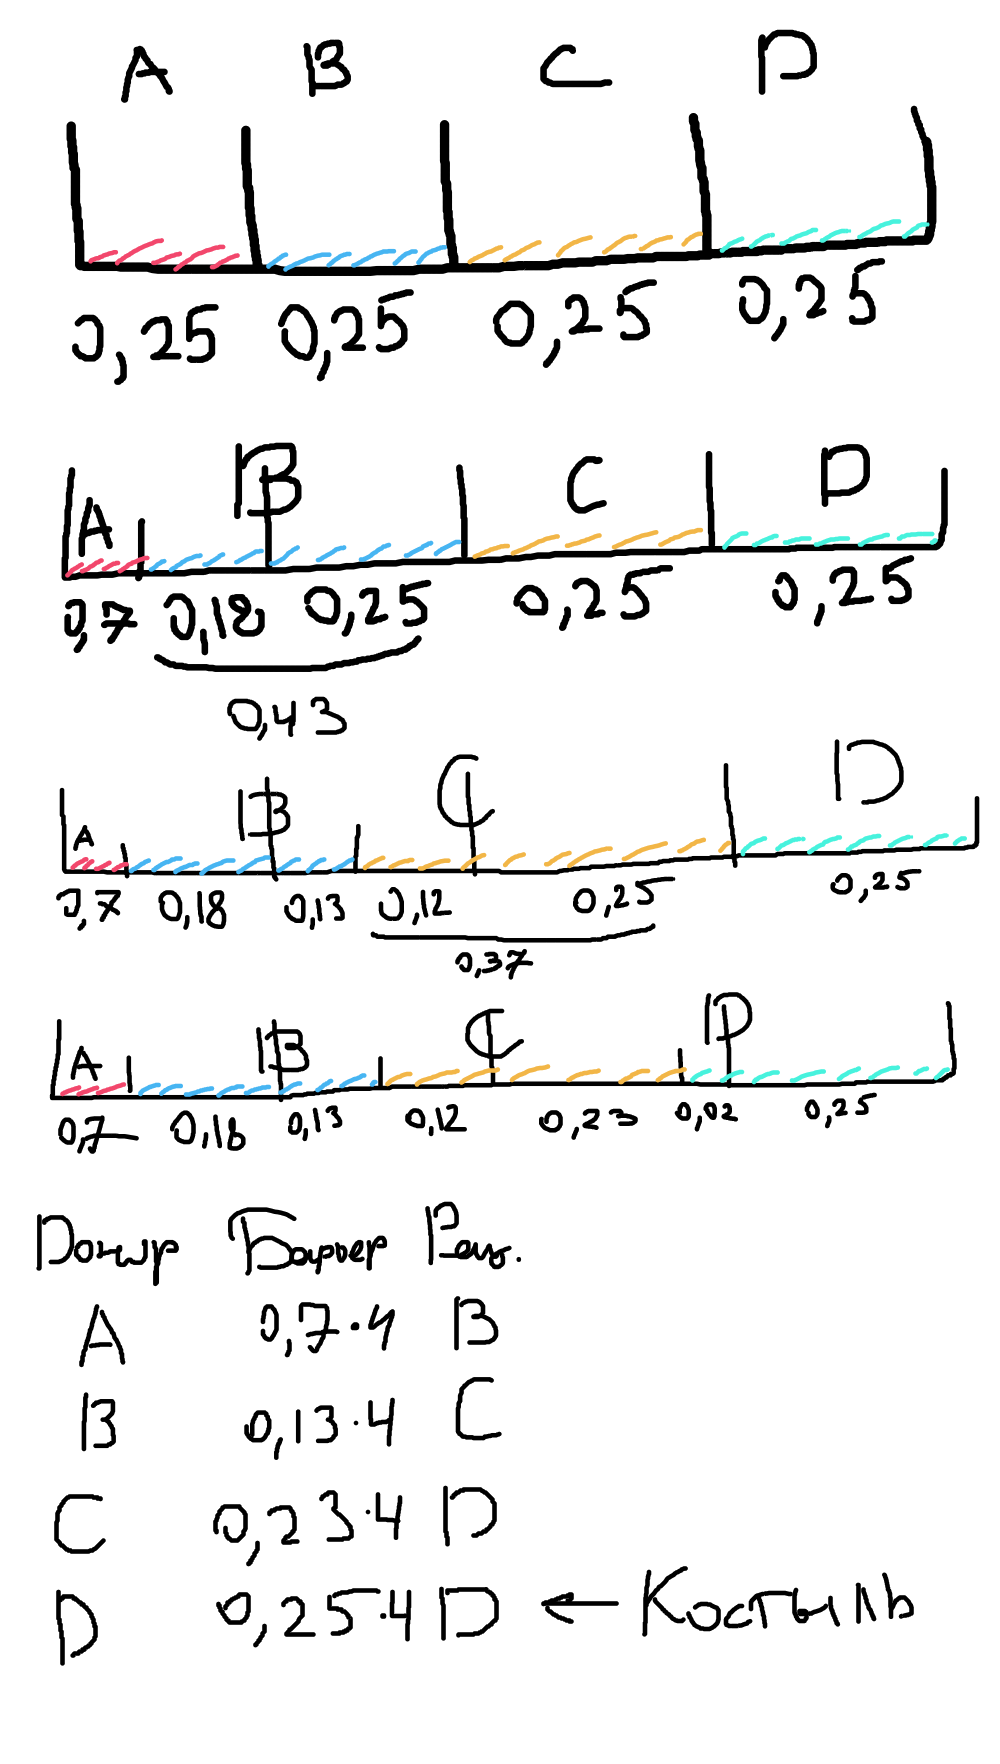
\includegraphics[scale=1.3]{pics/walker.png}
          \centering
      \end{figure}
  \end{Example}
\end{document}
